% JUMP TO LINE 60, 75
\documentclass{article}
\usepackage[letterpaper,portrait,top=0.4in, left=0.6in, right=0.6in, bottom=1in]{geometry}

\usepackage{amsmath, amsfonts, amsthm, amssymb}
\usepackage{graphicx, float}
\usepackage{mathtools}
\usepackage{titlesec}
\usepackage{interval}
\usepackage{hyperref}
\usepackage{siunitx}
\usepackage{titling}
\usepackage{vwcol}
\usepackage{setspace}
\usepackage{empheq}
\usepackage{cancel}
\usepackage{esdiff}
\usepackage{multicol}
\usepackage{mdframed}
\usepackage{esdiff}
\usepackage{tikzsymbols}
\usepackage{multicol}
\usepackage{tikz}
\usepackage{varwidth}
\usepackage{parskip}
\usepackage{pgfplots}
\usepackage{mlmodern}
\pgfplotsset{compat=1.18}
\intervalconfig {
	soft open fences
}

\newcommand{\alignedintertext}[1]{%
  \noalign{%
    \vtop{\hsize=\linewidth#1\par
    \expandafter}%
    \expandafter\prevdepth\the\prevdepth
  }%
}

\usetikzlibrary{positioning}
\usetikzlibrary{angles,quotes}

\newtheorem{lemma}{Lemma}

\newcommand*{\problem}[1]{\section*{Problem #1}}
\newcommand*{\aps}{\section*{AP Corner}}
\newcommand*{\deriv}[1][x]{\ensuremath{\dfrac{\mathrm{d}}{\mathrm{d}#1}}}
\newcommand*{\floor}[1]{\ensuremath{\lfloor #1\rfloor}}
\newcommand*{\lheqzero}{\ensuremath{\underset{\text{L'H}}{\overset{\left[\frac00\right]}{=}}}}
\newcommand*{\lheqinfty}{\ensuremath{\underset{\text{L'H}}{\overset{\left[\frac{\infty}{\infty}\right]}{=}}}}

\DeclareMathOperator{\DNE}{DNE}
\DeclareMathOperator{\sgn}{sgn}

\DeclareMathOperator{\arccsc}{arccsc}
\DeclareMathOperator{\arcsec}{arcsec}
\DeclareMathOperator{\arccot}{arccot}

%opening

\title{\vspace*{-40pt}Multivariable Calculus Summer Assignment}
\author{Jayden Li}
\date{\today}
% \allowdisplaybreaks
\postdisplaypenalty=100000

\begin{document}
\setstretch{1.25}
\fontsize{12pt}{12pt}\selectfont
\setlength{\abovedisplayskip}{\abovedisplayskip/2}
\setlength{\belowdisplayskip}{\belowdisplayskip/2}
\setlength{\parindent}{0pt}
\setlength{\parskip}{2ex plus 0.5ex minus 0.2ex}
\maketitle

\problem{1}
\begin{itemize}
	\item[(ab)]
		\phantom{}
		\vspace{-\parskip}

		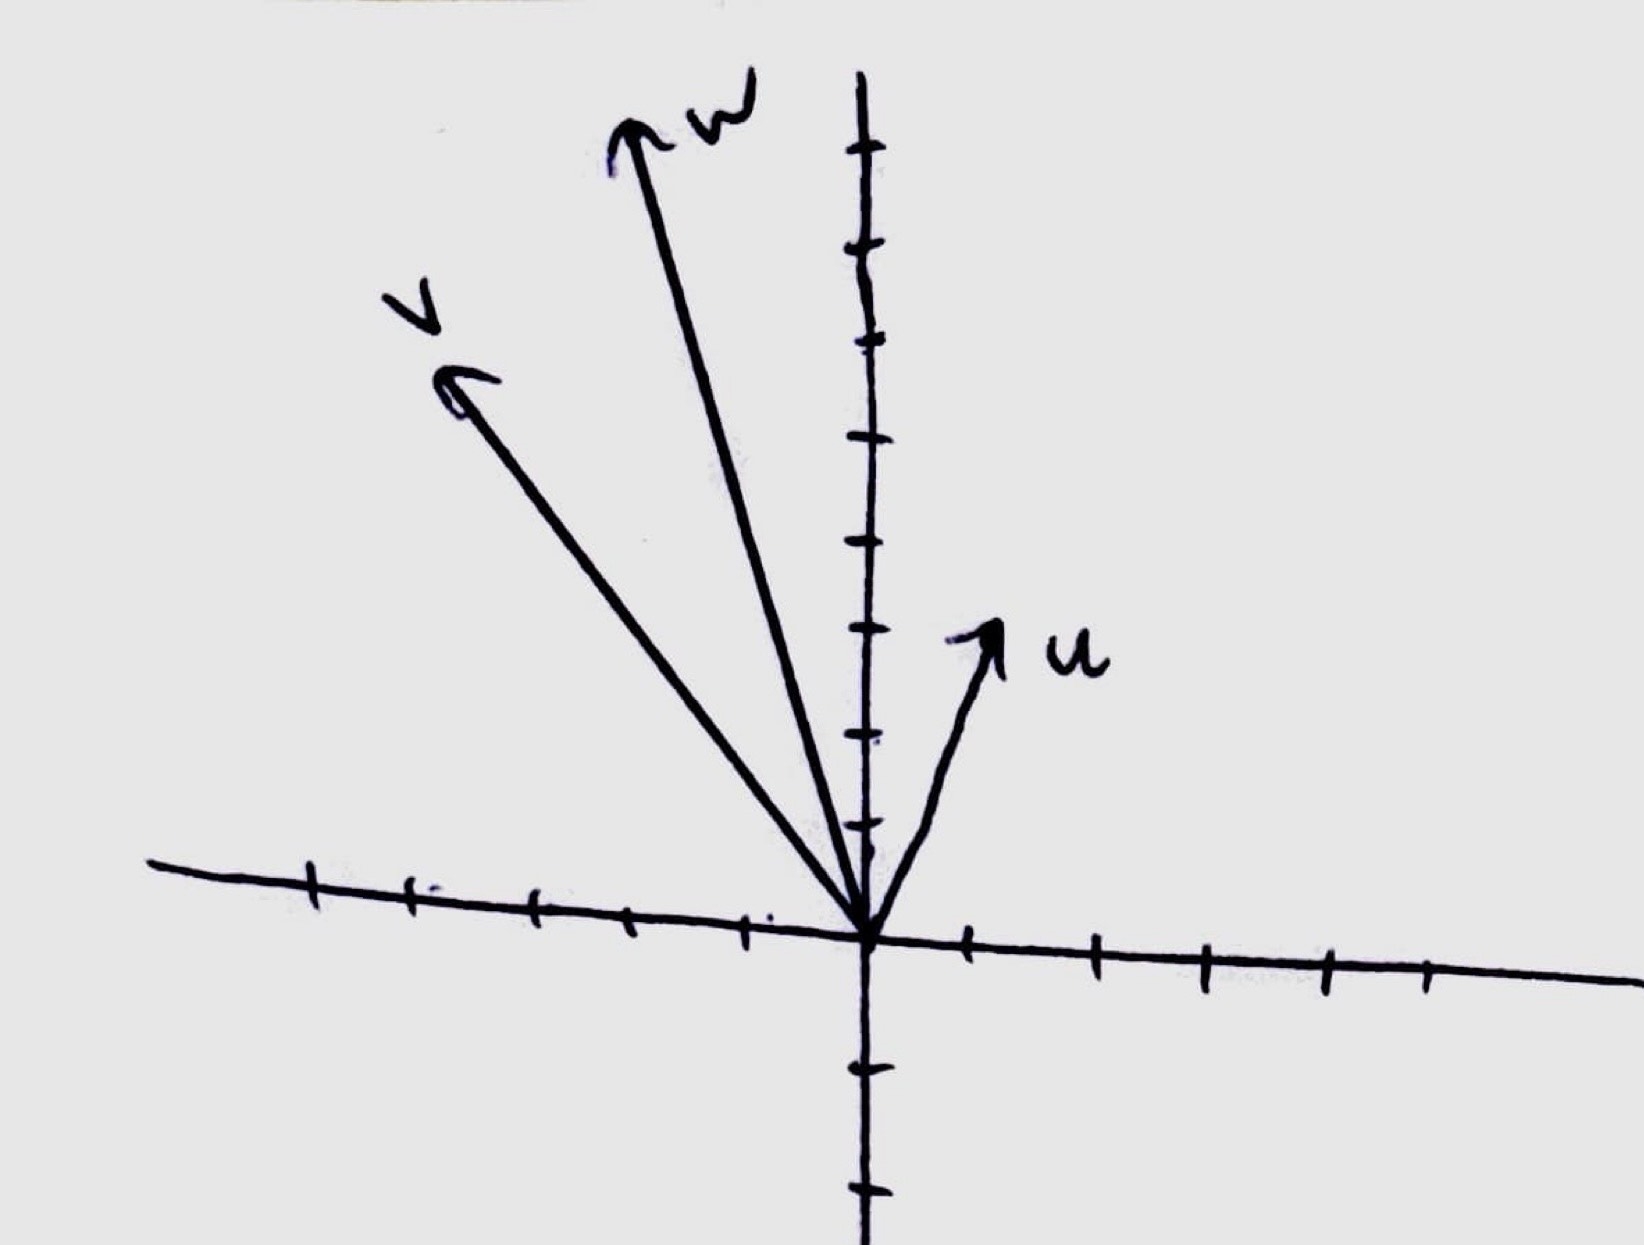
\includegraphics[width=0.5\linewidth]{q1.jpeg}

	\item[(c)]
		$\begin{aligned}[t]
			\left\lVert u \right\rVert
			&=\sqrt{(1)^2+(3)^2}
			=\sqrt{1+9}
			=\boxed{\sqrt{10}} \\
			\left\lVert v \right\rVert 
			&=\sqrt{(-4)^2+(5)^2}
			=\sqrt{16+25}
			=\boxed{\sqrt{41}} \\
			\left\lVert w \right\rVert 
			&=\left\lVert \left< -3,8 \right> \right\rVert 
			=\sqrt{(-3)^2+(8)^2}
			=\sqrt{9+64}
			=\boxed{\sqrt{73}}
		\end{aligned}$

	\item[(d)]
		$\begin{aligned}[t]
		    u+v 
			&=\left< 1,3 \right>+\left< -4,5 \right>
			=\boxed{\left< -3,8 \right>} \\
			\left\lVert u+v \right\rVert 
			&=\left\lVert w \right\rVert 
			=\boxed{\sqrt{73}}
		\end{aligned}$

	\item[(e)] Vectors $a$ and $b$ must be orthogonal, which is exactly when $a^Tb=b^Ta=a\cdot b=0$.
	\begin{proof}
		Let $a$ and $b$ be vectors such that $\left\lVert a\right\rVert+\lVert b \rVert=\lVert a + b\rVert$. By definition, this is equivalent to:
		\begin{align*}
		    a^Ta+b^Tb
			&=(a+b)^T(a+b) \\
			&=\left(a^T+b^T\right)(a+b) \\ 
			\cancel{a^Ta}+\cancel{b^Tb}
			&=\cancel{a^Ta}+a^Tb+b^Ta+\cancel{b^Tb} \\
			0&=a^Tb+b^Ta
		\end{align*}
		The dot product is commutative: $a\cdot b=b\cdot a$ so $a^Tb=b^Ta$.

		Thus we must have $2a^Tb=0 \iff \boxed{a^Tb=a\cdot b=0\iff \text{$a$ and $b$ are orthogonal}}$ for $\left\lVert a \right\rVert+\lVert b \rVert=\lVert a+b \rVert$, which is the equality case of the triangle inequality/Pythagorean theorem.
	\end{proof}
\end{itemize}

\problem{2}
\begin{itemize}
	\item[(abc)]
		$\begin{aligned}[t]
		    -v 
			&=-\left< -4,5 \right>
			=\boxed{\left< 4,-5 \right>} \\
			u+(-v)
			&=\left< 1,3 \right>+\left< 4,-5 \right>
			=\boxed{\left< 5,-2 \right>}
		\end{aligned}$

		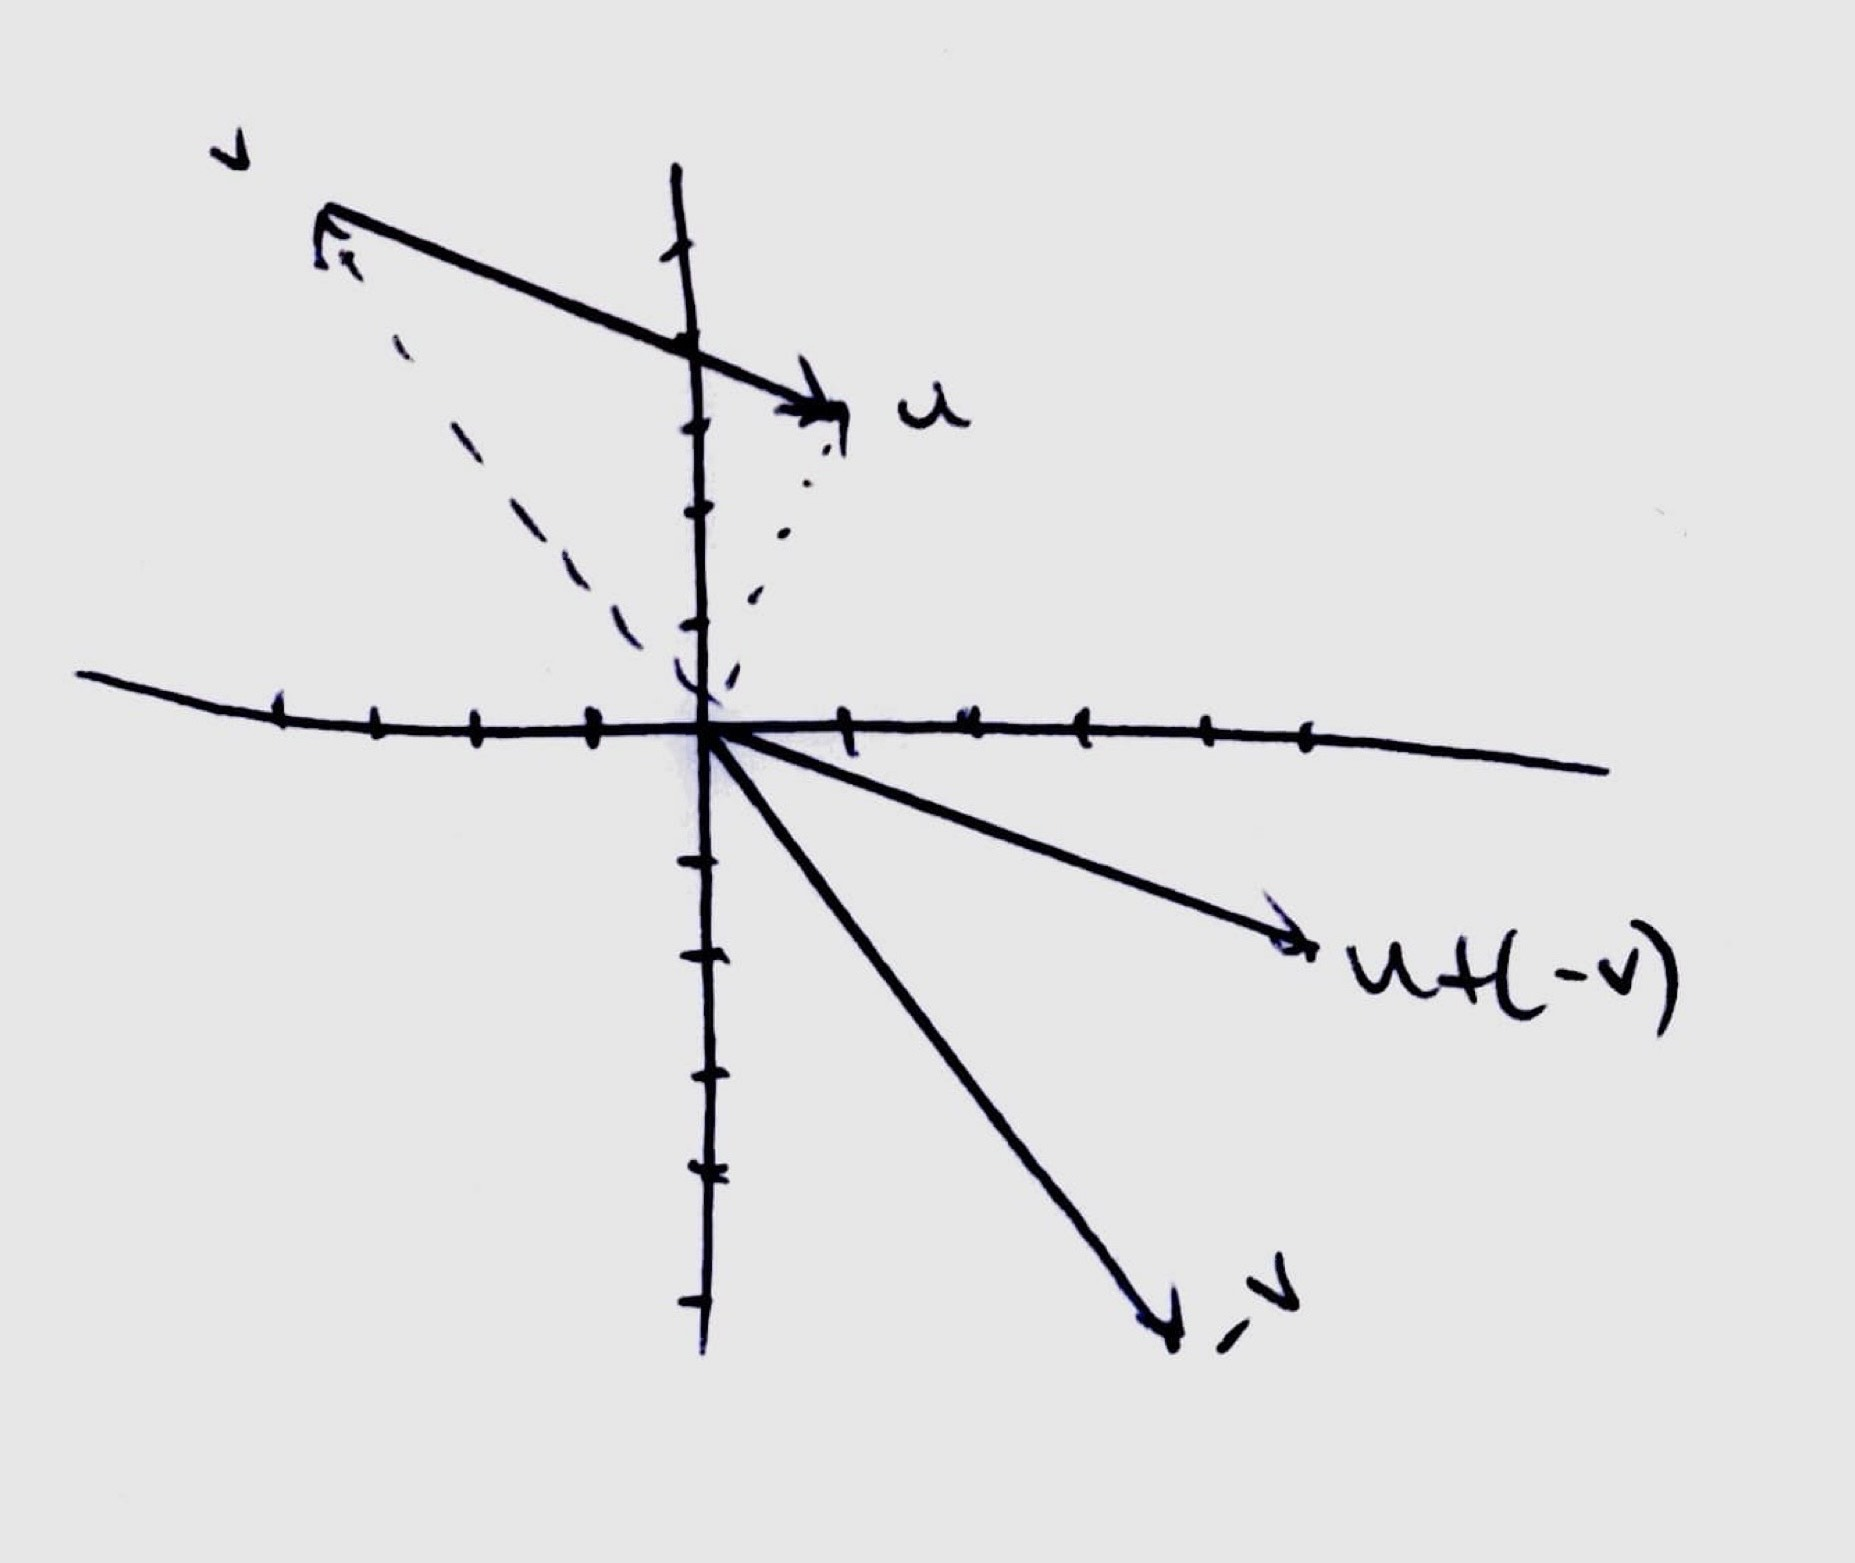
\includegraphics[width=0.6\linewidth]{q2.jpeg}

	\item[(c)]
		This vector is the same as the vector found in part (b).
\end{itemize}

\problem{3}
\begin{itemize}
	\item[(a)] $AB$ is equivalent to $CD$.
	\item[(b)] $BC$ is equivalent to $AD$.
	\item[(c)] $\displaystyle AM=\frac{AC}{2}=\frac{AB+BC}{2}$.
	\item[(d)] $\displaystyle AB+BC-AC=AC-AC=0$.
\end{itemize}


\problem{4}
\begin{minipage}[t]{0.4\linewidth}
	\begin{tikzpicture}[
		baseline=(current bounding box.north),
		ang/.style={draw, angle eccentricity=1.5,angle radius=0.6cm}
	]	
		\draw 
		(-1.5,2) coordinate[label=above left:{$A(-3,4)$}](A)
		-- (1,3) coordinate[label=above:{$B(2,6)$}](B)
		-- (2,-3) coordinate[label=right:{$C(4,-6)$}](C)
		-- cycle;
	\end{tikzpicture}
\end{minipage}
\begin{minipage}[t]{0.59\linewidth}
\begin{itemize}
	\item[(a)]
		$\begin{aligned}[t]
			AB&=B-A=\left< 2-(-3), 6-4 \right>=\boxed{\left< 5,2 \right>} \\
			BC&=C-B=\left< 4-2,-6-6 \right>=\boxed{\left< 2,-12 \right>} \\
			CA&=A-C=\left< -3-4, 4-(-6) \right>=\boxed{\left< -7, 10 \right>}
		\end{aligned}$
	
	\item[(b)]
		$AB+BC+CA=\boxed{\left< 0, 0 \right>}$
		\vspace{6pt}

	\item[(c)]
		$\begin{aligned}[t]
			&{}\frac12 AC-\frac12 AB
			=\frac12 CA-\frac12 AB \\
			={}&-\frac12 \left< -7,10 \right>-\frac12 \left< 5,2 \right>
			=\left< \frac{7}{2}, -5 \right>-\left< \frac52,1 \right> \\
			={}&\left< \frac72-\frac52, -5-1 \right>
			=\boxed{\left< 1,-6 \right>}
			=\frac12 BC
		\end{aligned}$
\end{itemize}
\end{minipage}

\begin{itemize}
	\item[(d)]
		$\begin{aligned}[t]
			AC 
			&=C-A 
			=\left< 4,-6,5 \right>-\left< -3,4,2 \right>
			=\left< 7, -10, 3 \right> \\
			AB 
			&=B-A 
			=\left< 2,6,-1 \right>-\left< -3,4,2 \right>
			=\left< 5,2,-3 \right> \\
			BC 
			&=C-B 
			=\left< 4,-6,5 \right>-\left< 2,6,-1 \right>
			=\left< 2,-12,6 \right> \\
		    \frac12AC-\frac12AB
			&=\frac12 \left< 7,-10,3 \right>-\frac{1}{2}\left< 5,2,-3 \right>
			=\left< \frac72,-5,\frac32 \right>-\left< \frac52,1,-\frac32 \right> \\
			&=\left< \frac72-\frac52, -5-1, \frac32+\frac32 \right>
			=\boxed{\left< 1, -6, 3 \right>}
			=\frac12 \left< 2,-12,6 \right>
			=\frac12 BC
		\end{aligned}$

		$AC/2-AB/2$ is still a scalar multiple of $BC$.
\end{itemize}


\problem{5}
\begin{itemize}
	\item[(a)] \boxed{n=\left< s,-r \right>}.

	\item[(b)] $m\cdot n=rs+s(-r)=rs-rs=\boxed{0}$.

	\item[(c)] $(2n)\cdot (-3m)=\left< 2s,-2r \right>\cdot \left< -3r,-3s \right>=(2s)(-3r)+(-2r)(-3s)=-6sr+6rs=0$. Geometrically, this means $2n$ and $-3m$ are also perpendicular.

	\item[(d)] $u\cdot v=\left< 1,3 \right>\cdot \left< -4,5 \right>=(1)(-4)+(3)(5)=-4+15=11$ so $u$ and $v$ are not perpendicular.

	\item[(e)] The dot product is commutative.

	\begin{proof}
		Let $a=(a_1,a_2,\ldots,a_n)$ and $b=(b_1,b_2,\ldots,b_n)$ be vectors in $\mathbb R^n$, and $a_i,b_i\in\mathbb R$. Then:
		\begin{align*}
		    a\cdot b 
			&=a_1b_1+a_2b_2+\ldots+a_nb_n
			=\sum_{k=1}^{n}a_kb_k \\
		    b\cdot a
			&=b_1a_1+b_2a_2+\ldots+b_na_n
			=\sum_{k=1}^{n}b_ka_k
			=\sum_{k=1}^{n}a_kb_k
		\end{align*}
		Scalar multiplication $a_kb_k$ is commutative. Since $a\cdot b=b\cdot a$, the dot product is commutative.
	\end{proof}
	\begin{proof}
		Alternatively, let $a,b$ be vectors in $\mathbb R^n$. The dot product is defined as:
		\begin{align}
		    a\cdot b
			&=\left\lVert a \right\rVert \lVert b \rVert \cos \theta \\
		    b\cdot a
			&=\left\lVert b \right\rVert \lVert a \rVert \cos \theta
		\end{align}
		where $\theta$ is the angle between vectors $a$ and $b$. Since vector norms $\left\lVert a \right\rVert$ and $\lVert b \rVert$ are scalar values, and scalar multiplication is commutative, we have $\lVert a \rVert \lVert b \rVert=\lVert b \rVert \lVert a \rVert$. Since $\theta$ remains the same in (1) and (2), as the angle between vectors do not change, $a\cdot b$ must equal $b\cdot a$.
	\end{proof}
\end{itemize}

\problem{6}
\begin{itemize}
	\item[(a)] DeGray's displacement vector $\boxed{v=\left< 10,30,15 \right>}$. The distance to his starting point is $\left\lVert v \right\rVert =\sqrt{(10)^2+(30)^2+(15)^2}=\sqrt{100+900+225}=\sqrt{1225}=35$ meters.

	\item[(b)] Seltzer's displacement vector $\boxed{w=\left< 40,-60,-10 \right>}$. The straight line distance from DeGray to Seltzer is $\boxed{w-v}=\left< 30,-90,-25 \right>$.
	
	\item[(c)]
		$\begin{aligned}[t]
			D
			&=\left\lVert \left< 50\cdot 10^6, 20\cdot 10^6, 30\cdot 10^6, 80\cdot 10^6 \right> \right\rVert
			=\sqrt{\left(50\cdot 10^6\right)^2+\left(20\cdot 10^6\right)^2+\left(30\cdot 10^6\right)^2+\left(80\cdot 10^6\right)^2} \\
			&=\sqrt{10^{12}\left( 50^2+20^2+30^2+80^2 \right)}
			=\sqrt{10^{12}}\sqrt{2500+400+900+6400} \\
			&=10^6 \sqrt{100 \left( 25+4+9+64 \right)}
			=10^6 \sqrt{100} \sqrt{102}
			=10^7 \sqrt{102}
		\end{aligned}$

		The ship needs to travel \boxed{10^7 \sqrt{102} \text{ meters}} to return to the sun.
\end{itemize}

\problem{7}
\begin{itemize}
	\item[(a)] The vertices of the cube are: $\left( 0,0,0 \right),\left( 2,0,0 \right), \left( 0,2,0 \right), \left( 0,0,2 \right), \left( 2,2,0 \right), \left( 2,0,2 \right), \left( 0,2,2 \right), \left( 2,2,2 \right)$. Also, $A=\left( 2,1,0 \right), B=\left( 2,2,1 \right), C=\left( 1,2,2 \right)$.

	\item[(b)] $OA=\left< 2,1,0 \right>, OB=\left< 2,2,1 \right>, OC=\left< 1,2,2 \right>$.

	\item[(c)] $BA=\boxed{OA-OB}=\left< 0,-1,-1 \right>$ and $BC=\boxed{OC-OB}=\left< -1,0,1 \right>$.

	\item[(d)] $BA\cdot BC=\left< 0,-1,-1 \right>\cdot \left< -1,0,1 \right>=(0)(-1)+(-1)(0)+(-1)(1)=\boxed{-1}$. This means $BA$ and $BC$ are not perpendicular.

	\item[(e)]
		$\begin{aligned}[t]
			\lVert OA \rVert &=\sqrt{(2)^2+(1)^2+(0)^2}=\sqrt{4+1+0}=\boxed{\sqrt{5}} \\
			\lVert OB \rVert &=\sqrt{(2)^2+(2)^2+(1)^2}=\sqrt{4+4+1}=\sqrt{9}=\boxed{3} \\
			\lVert OC \rVert &=\sqrt{(1)^2+(2)^2+(2)^2}=\sqrt{1+4+4}=\sqrt{9}=\boxed{3} \\
			\lVert BA \rVert &=\sqrt{(0)^2+(-1)^2+(-1)^2}=\sqrt{0+1+1}=\boxed{\sqrt{2}} \\
			\lVert BC \rVert &=\sqrt{(-1)^2+(0)^2+(1)^2}=\sqrt{1+0+1}=\boxed{\sqrt{2}}
		\end{aligned}$

	\item[(f)]
		$\begin{aligned}[t]
		    BA-BC
			&=\left< 0,-1,-1 \right>-\left< -1,0,1 \right>
			=\boxed{\left< 1,-1,-2 \right>} \\
			\lVert BA-BC \rVert 
			&=\lVert \left< 1,-1,-2 \right> \rVert 
			=\sqrt{(1)^2+(-1)^2+(-2)^2}
			=\sqrt{1+1+4}
			=\boxed{\sqrt{6}}
		\end{aligned}$

	\item[(g)]
		By the definition of the dot product, we have $BA\cdot BC=\lVert BA \rVert \lVert BC \rVert \cos \theta$, where $\theta$ is the angle between vectors $BA$ and $BC$, which equals $\angle ABC$.
		\begin{gather*}
			BA\cdot BC=\lVert BA \rVert \lVert BC \rVert \cos \theta \\
			\implies -1=\sqrt{2}\sqrt{2}\cos \theta 
			\implies -\frac12=\cos\theta
			\implies \theta=\arccos\left(-\frac12\right)
			=\boxed{\frac{2\pi}{3}}
		\end{gather*}
\end{itemize}

\problem{8}
\begin{equation*}
    r(t)=\left<2\cos t, 2\sin t\right>
\end{equation*}
\begin{itemize}
	\item[(a)] By the Pythagorean identity $\cos^2\theta+\sin^2\theta=1$:
		\begin{equation*}
		    \left\lVert r(t) \right\rVert
			=\sqrt{\left(2\cos t\right)^2+\left(2\sin t\right)^2}
			=\sqrt{4\cos^2t+4\sin^2t}
			=\sqrt{4}\sqrt{\cos^2t+\sin^2t}
			=2 \sqrt{1}
			=\boxed 2
		\end{equation*}
	
	\item[(b)]
		$\displaystyle 
			v(t)
			=r'(t)
			=\left<\deriv[t]2\cos t,\deriv[t]2\sin t\right>
			=\boxed{\left<-2\sin t,2\cos t\right>}
		$.
	
	\item[(c)]
		$\begin{aligned}[t]
		    v(t)\cdot r(t)
			&=\left<2\cos t, 2\sin t\right>\cdot \left<-2\sin t,2\cos t\right>
			=-4\cos t\sin t+4\sin t\cos t
			=0
		\end{aligned}$.

	\item[(d)]
		$\displaystyle 
			a(t)
			=v'(t)
			=\left<\deriv[t]\left[-2\sin t\right],\deriv[t]\left[2\cos t\right]\right>
			=\boxed{\left< -2\cos t, -2\sin t \right>}
		$.
	
	\item[(e)]
		$\displaystyle 
			a(t)
			=\left< -2\cos t, -2\sin t \right>
			=-1 \left< 2\cos t, 2\sin t \right>
			=-1r(t)
		$. $k=-1$.

	\item[(f)]
		\phantom{}

		\vspace{-\parskip}
		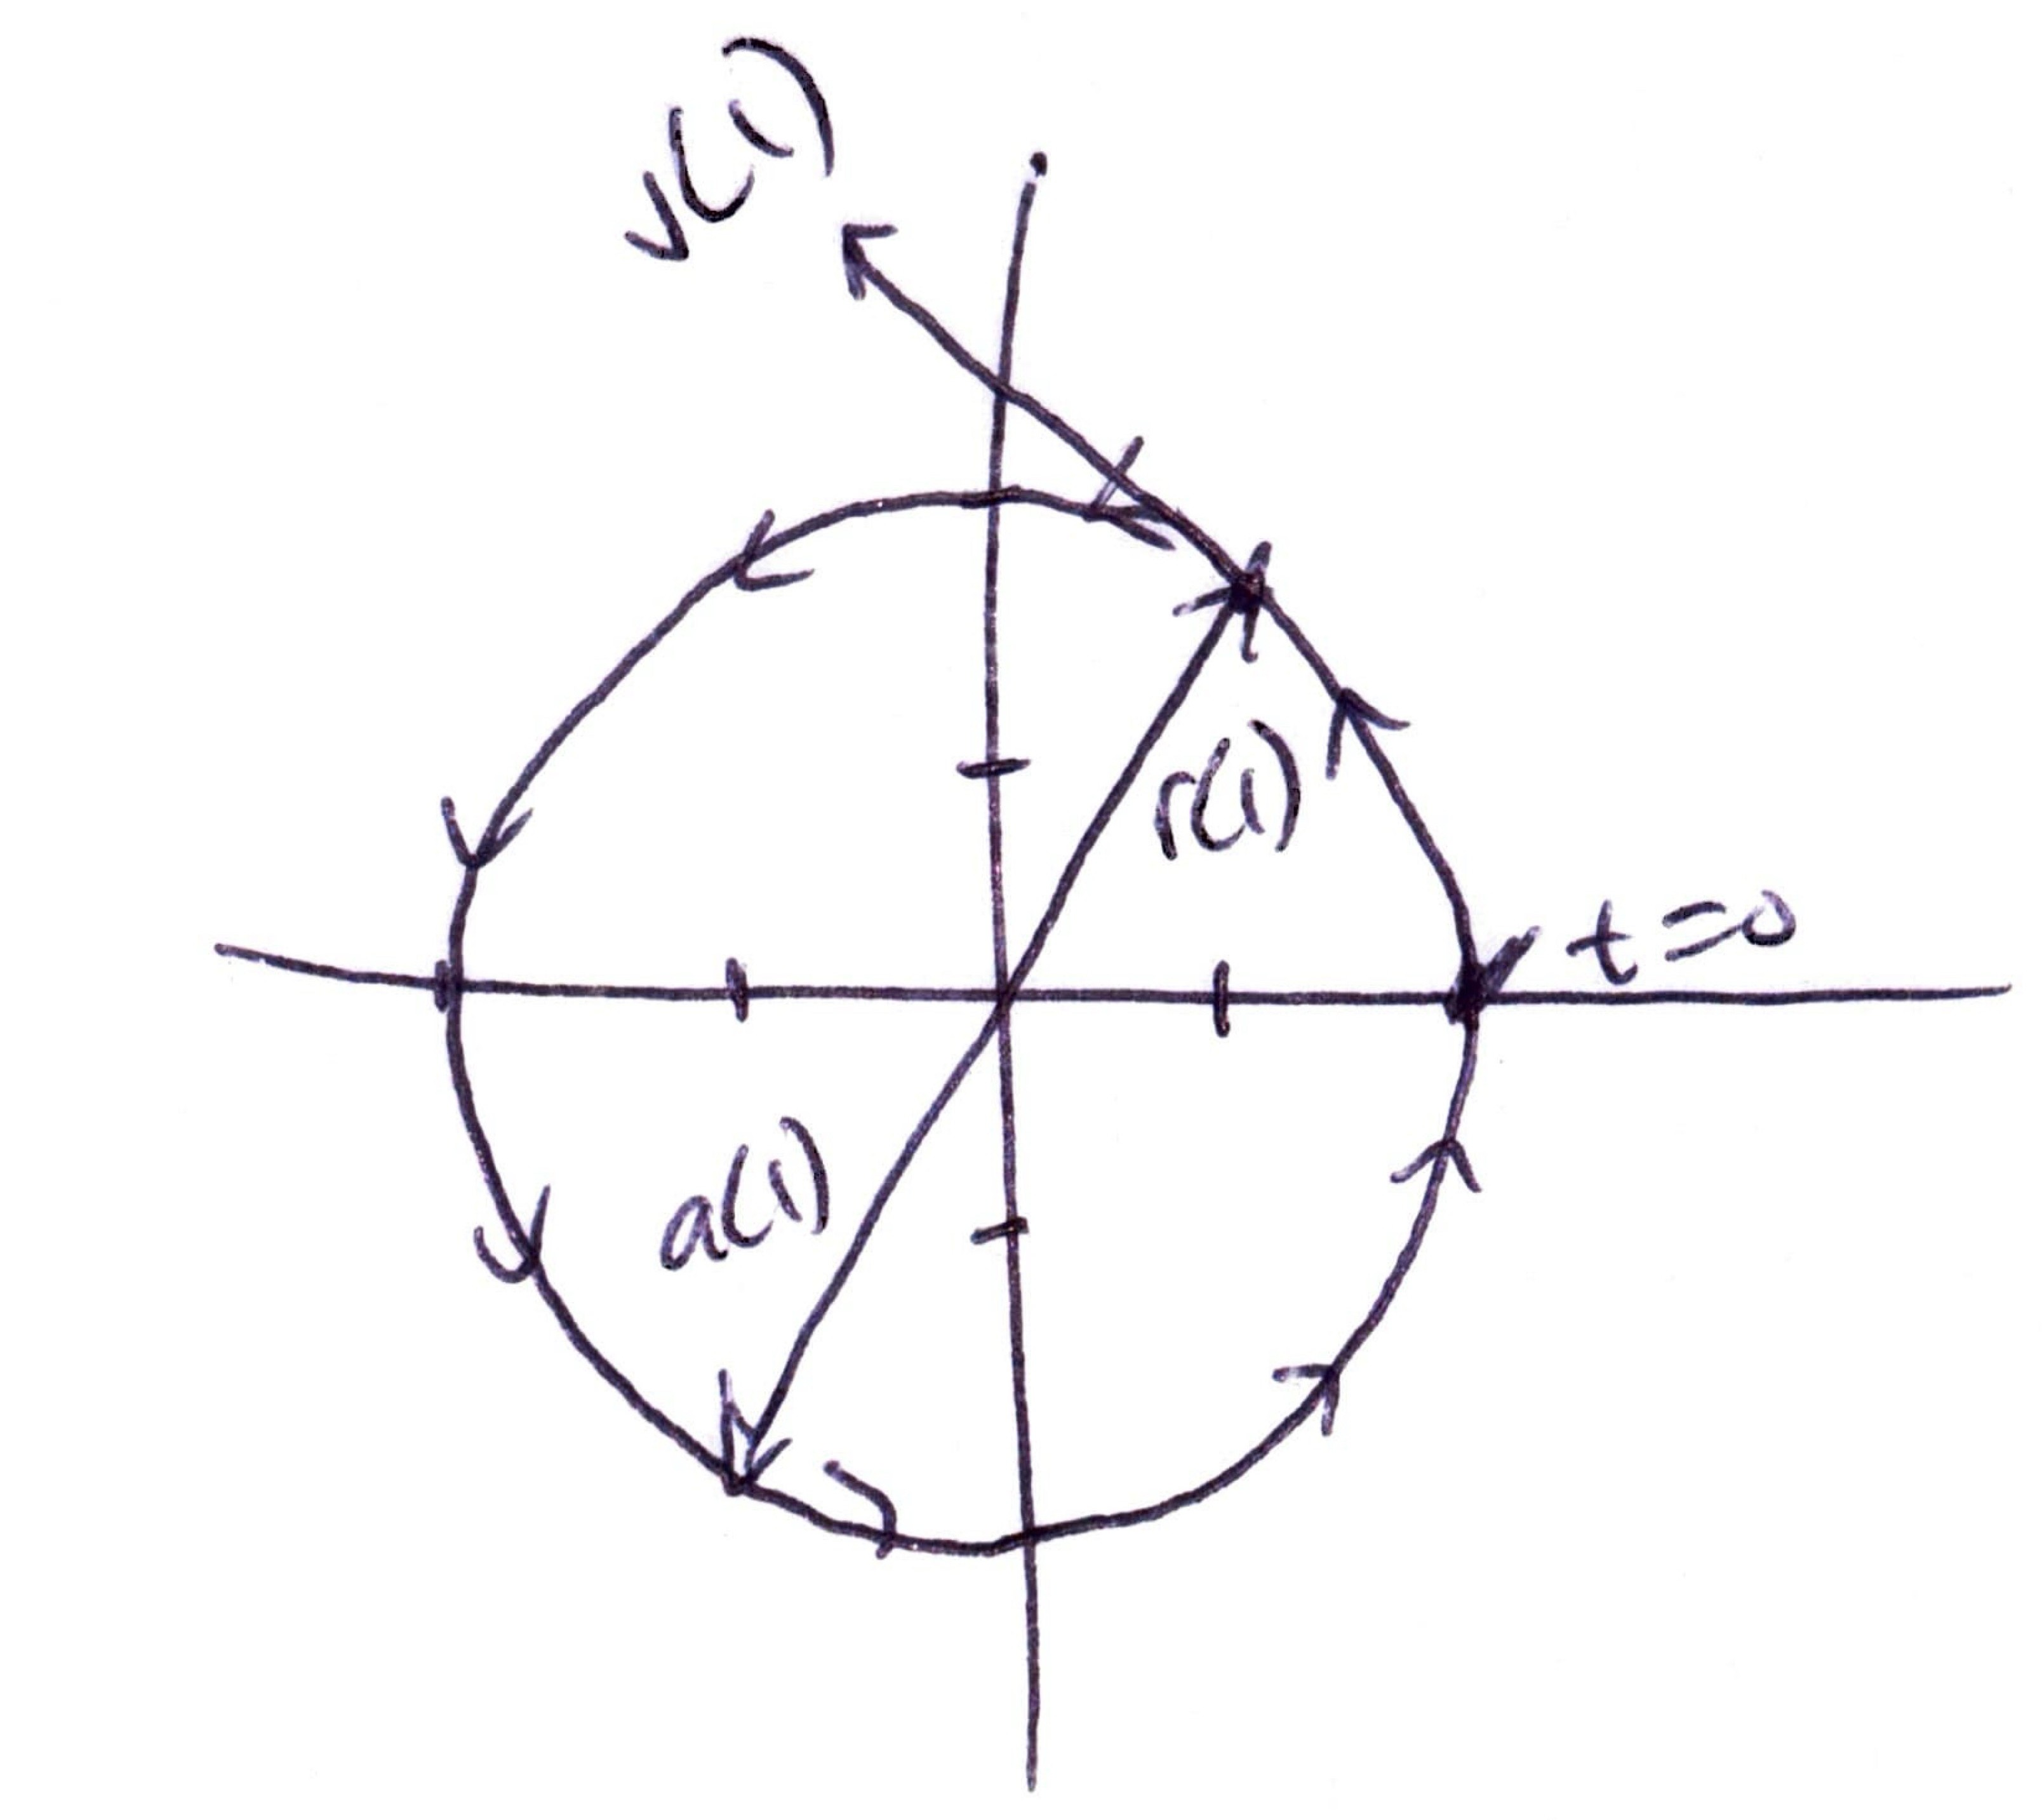
\includegraphics[width=0.4\linewidth]{q8.jpeg}
\end{itemize}


\problem{9}
\begin{itemize}
	\item[(a)] $u\cdot v=(1)(2)+(2)(10)+(-3)(5)=2+20-15=\boxed 7$.
	\item[(b)]
		\begin{align*}
			\underbrace{\begin{bmatrix}
				1 & 2 & -3 \\
				2 & 0 & -2
			\end{bmatrix}}_A
			\underbrace{\begin{bmatrix}
				2 & 0 & 1 \\
				10 & -2 & 3 \\
				5 & 5 & 2
			\end{bmatrix}}_B
			=\underbrace{\boxed{\begin{bmatrix}
				7 & -19 & 1 \\
				-6 & -10 & -2
			\end{bmatrix}}}_{AB}
		\end{align*}

	\item[(c)]
		The first column and first row of the result of matrix multiplication is $7$, which is the dot product between vectors $u$ and $v$. This is because $u$ is the first row of the left hand side matrix $A$, and $v$ is the first column of right hand side matrix $B$.

		In general, for any matrix product $AB$, we have:
		\begin{equation*}
			(AB)_{ij}=(\text{row $i$ of A})\cdot (\text{column $j$ of B})
		\end{equation*}
		where $(AB)_{ij}$ is the entry at the $i$th row and $j$th column of $C$.
\end{itemize}



\end{document}
